\documentclass{beamer}

\usepackage{beamerthemesplit}
\usepackage{tikz}
\usepackage{ocgx2}
\usepackage{amsmath,amsthm,amssymb,amscd, graphicx,bbm,xcolor}
\usepackage{array}
\usepackage{etoolbox}
\usepackage{mathtools}
\usepackage{subcaption}
\usepackage{multirow}

\DeclareMathOperator{\tr}{tr}
\newcommand{\E}{E}
\renewcommand{\P}{P}
\newcommand{\V}{Var}
\newcommand{\cov}{Cov}
\newcommand{\corr}{Corr}
\newcommand{\mean}[1]{\overline{#1}}
\newcommand{\cind}{\perp \!\!\! \perp}
\newcommand{\ones}{\mathbbm{1}}
\newcommand{\I}{N}
\newcommand{\Id}{E}
\newcommand{\e}{e}
\newcommand{\Q}{Q}
\newcommand{\eigval}{\lambda}
\renewcommand{\t}[1]{\tr(\Q^{#1})}
\newcommand{\rowmean}[1]{\overline{\phi}_{#1\cdot}}
\newcommand{\colmean}[1]{\overline{\phi}_{\cdot #1}}
\newcommand{\auchat}{\overline{\phi}_{\cdot \cdot}}
\newcommand{\coef}{c}
% \newtheorem{theorem}{Theorem}
% \newtheorem{proposition}{Proposition}
% \newtheorem{corollary}{Corollary}
% \newtheorem{lemma}{Lemma}
\mathtoolsset{showonlyrefs=true}
\newtoggle{speaktoggle}
\togglefalse{speaktoggle}
\newcommand{\speak}[1]{
  \iftoggle{speaktoggle}{
    {\tiny{\textcolor{red}{speak: #1}}\normalsize}
  }
  {}
}
\setbeamertemplate{footline}[frame number]

\title{Inference on the AUC with clustered data}
\author{Haben Michael}
\date{October 2021}

\AtBeginSection[] 
{
  \begin{frame}<beamer>
    \frametitle{Outline} 
    \tableofcontents[currentsection]  
  \end{frame}
}

\begin{document}



\begin{frame}
  \titlepage
\end{frame}





% \section{Introduction}
\begin{frame}
  \centering
  A motivating example
  \medskip
  \begin{columns}
    \begin{column}{.3\textwidth}
      Data: The Yale Prospective Longitudinal HIV Cohort
      \vspace{.2in}
      
      Problem: Evaluate CD4 as a predictor of blip status
    \end{column}
    \begin{column}{.7\textwidth}
      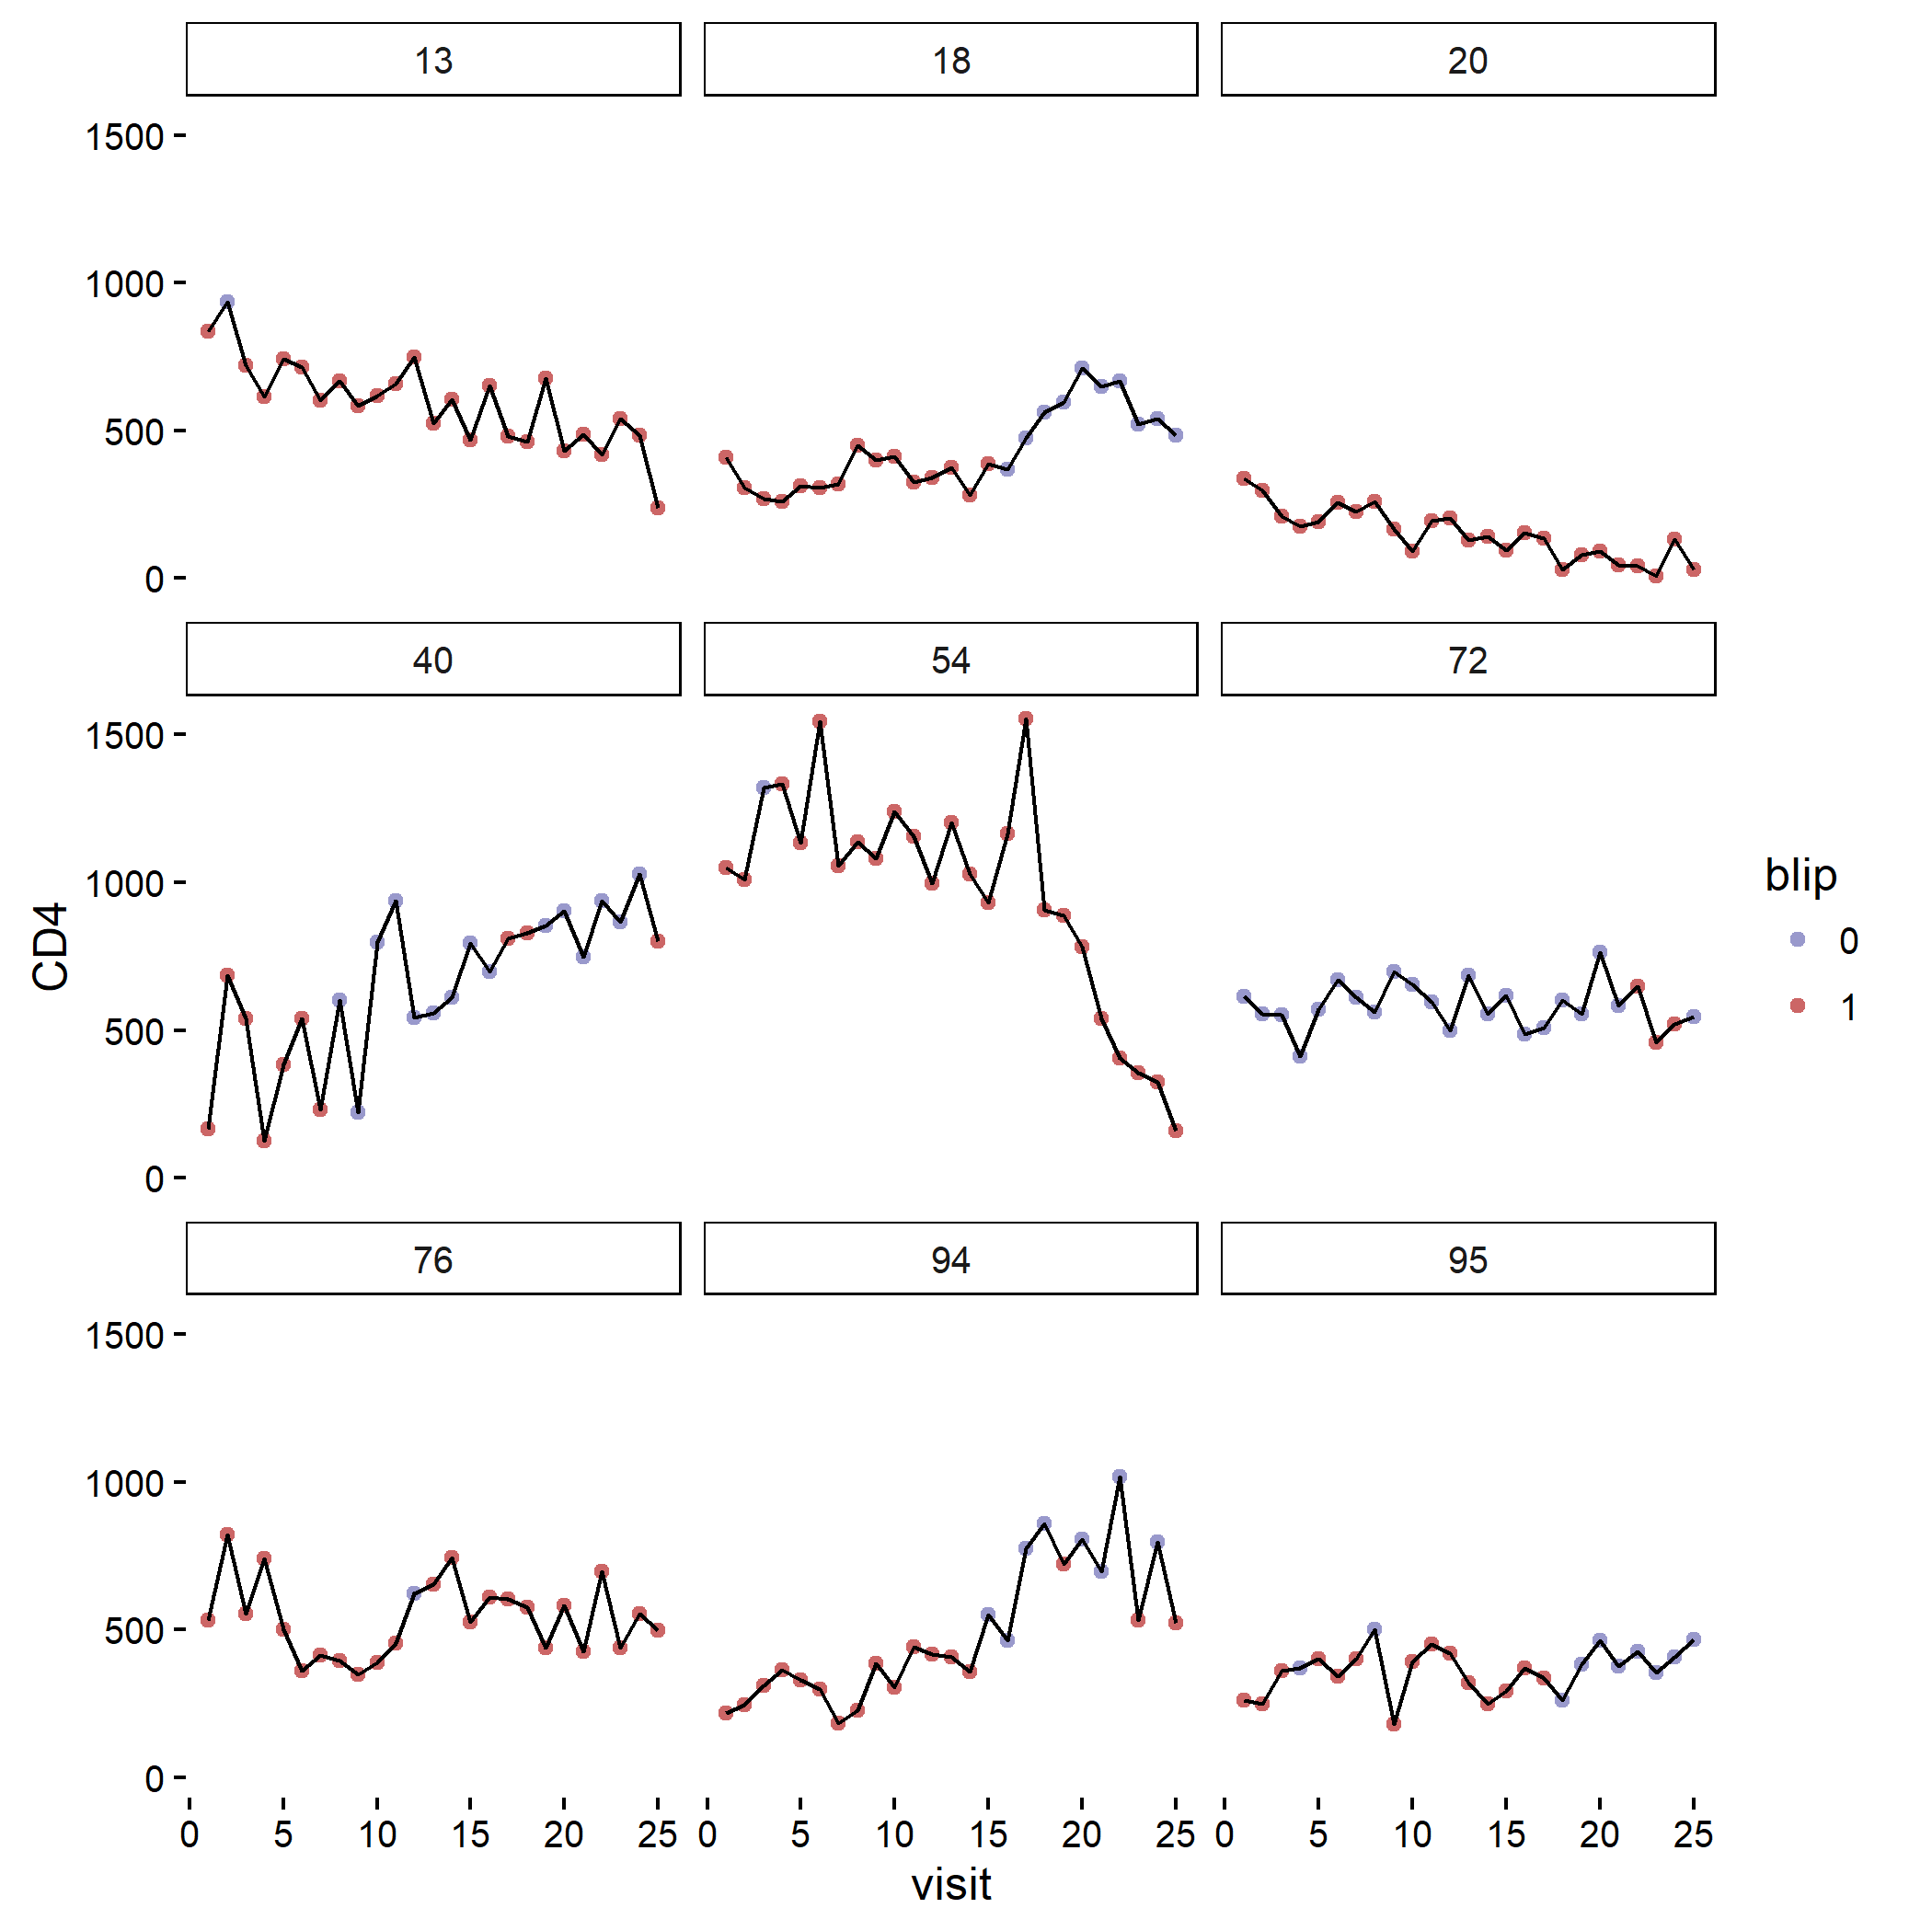
\includegraphics[width=\textwidth]{fig5.png}
    \end{column}
  \end{columns}
  
  % motivating example -- 
  % 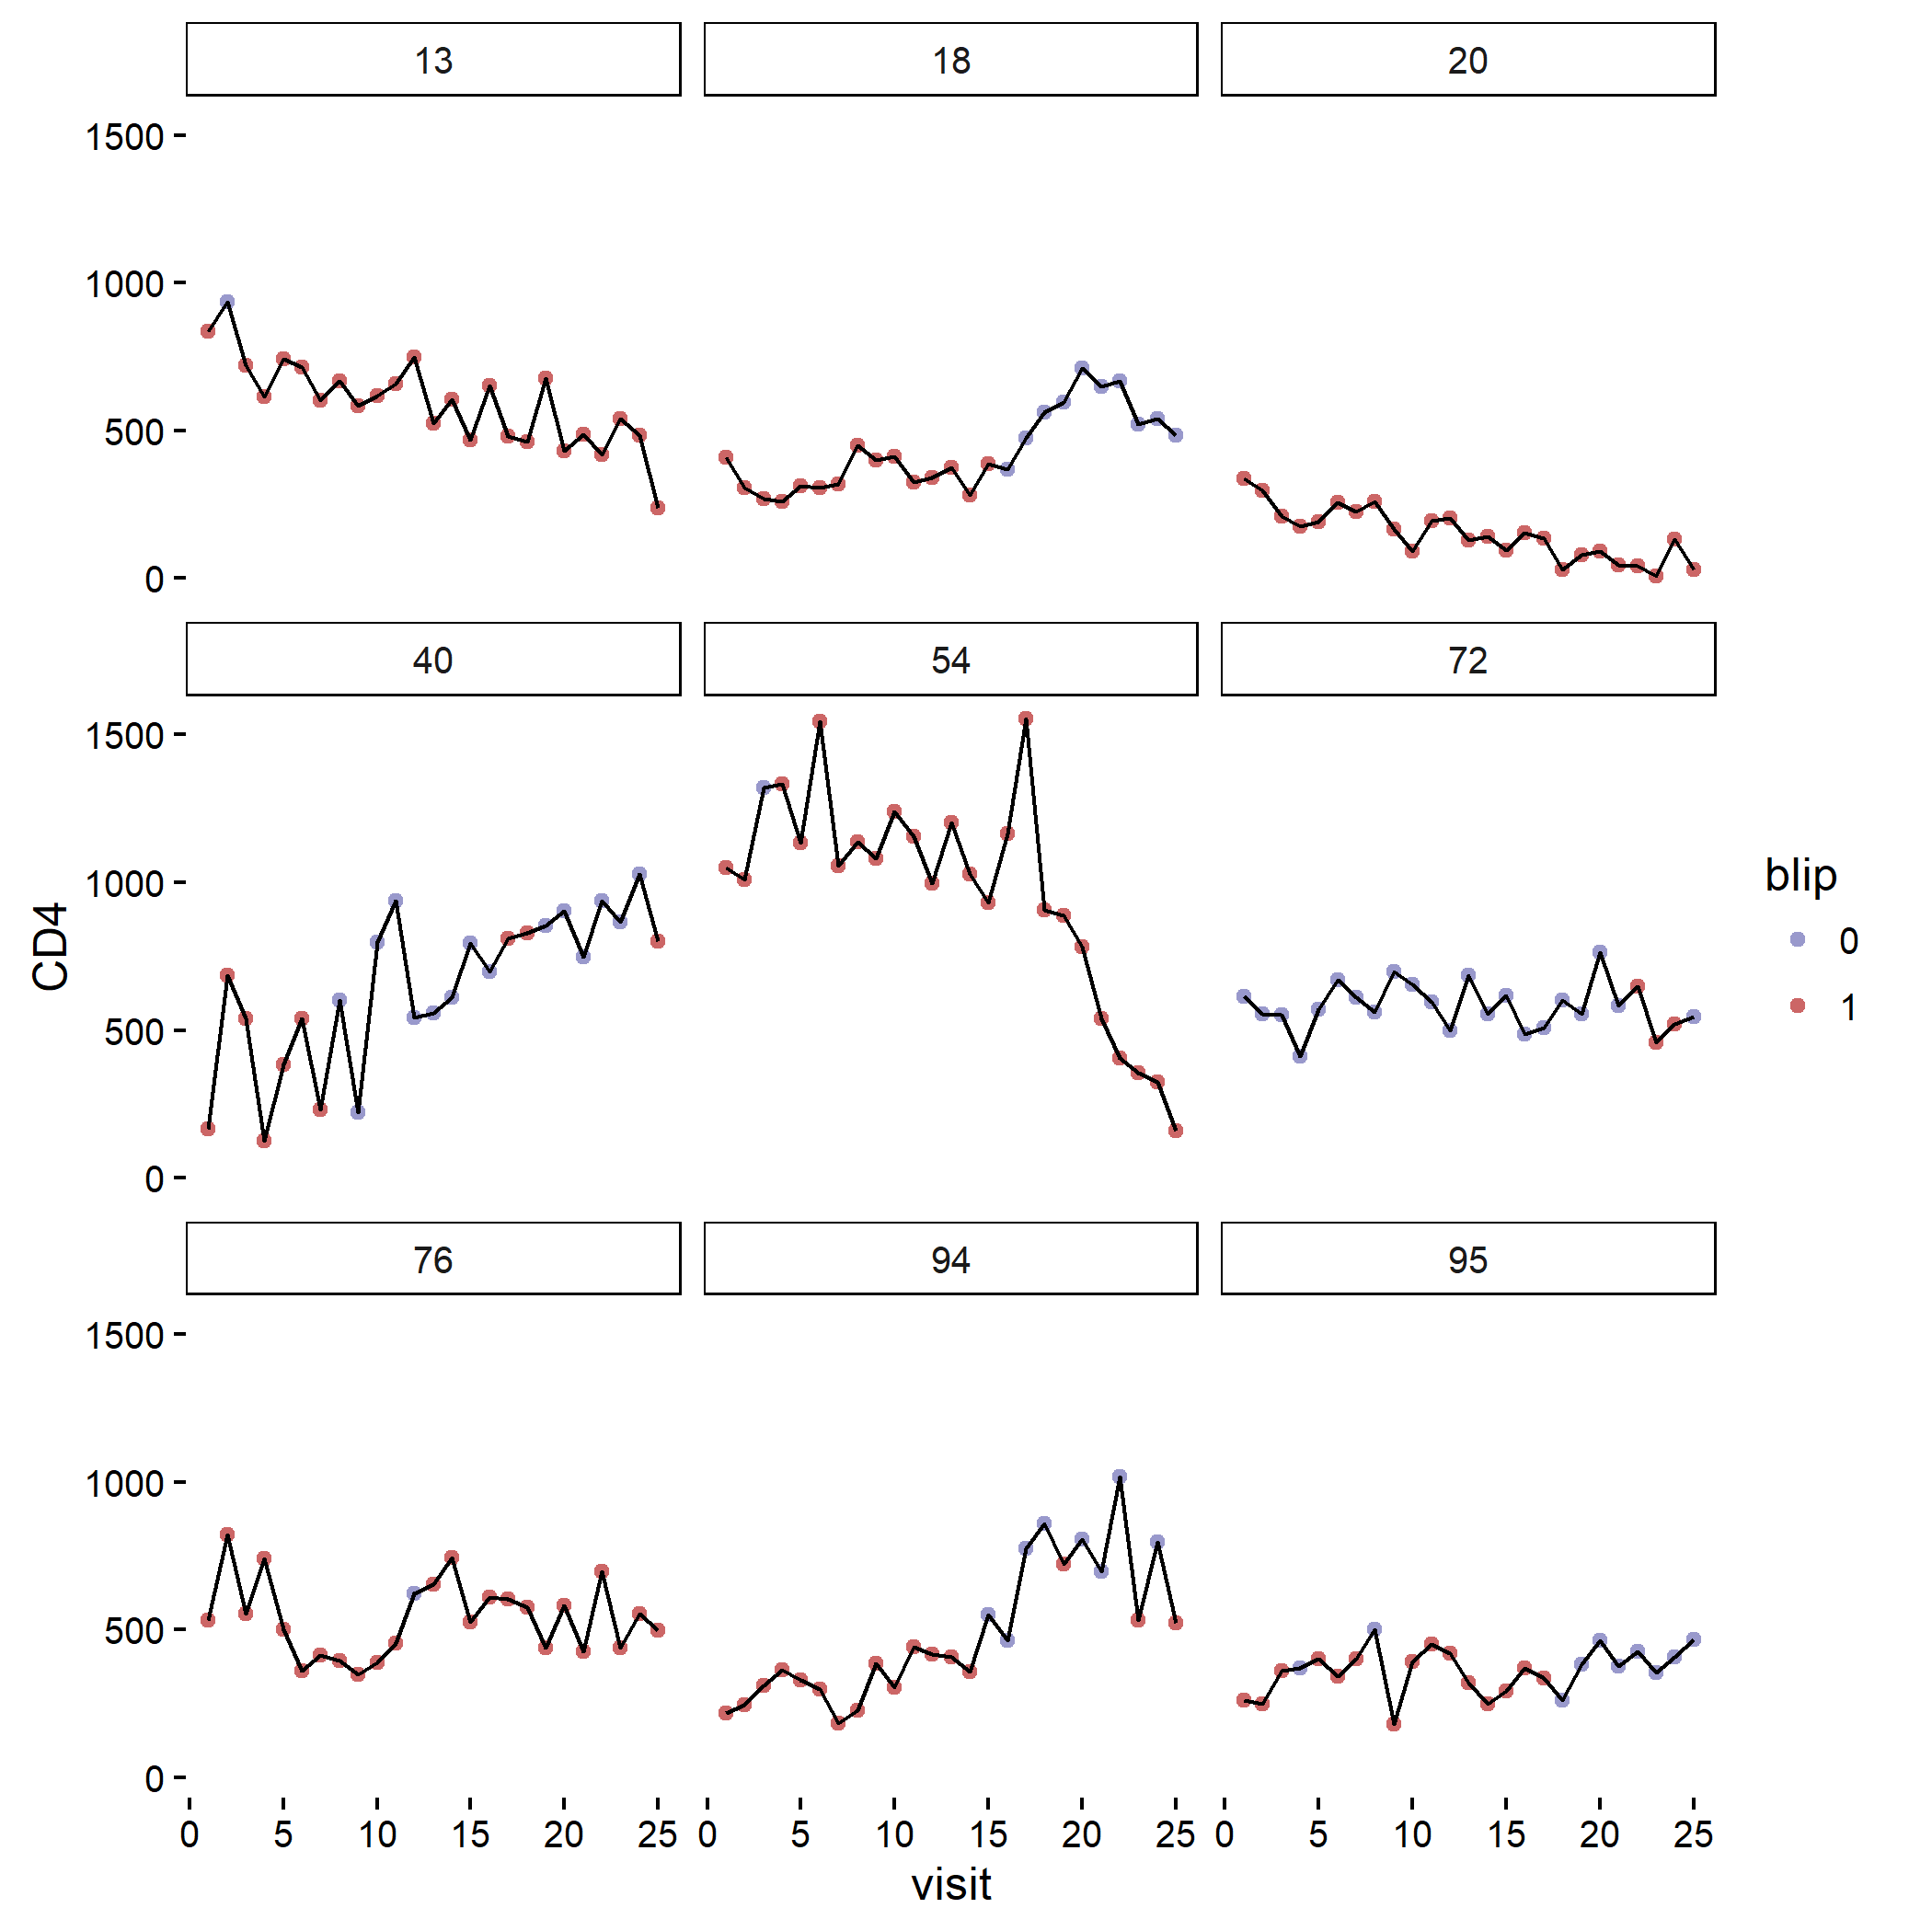
\includegraphics[scale=.4]{fig5.png}
\end{frame}
\begin{frame}
  \centering
  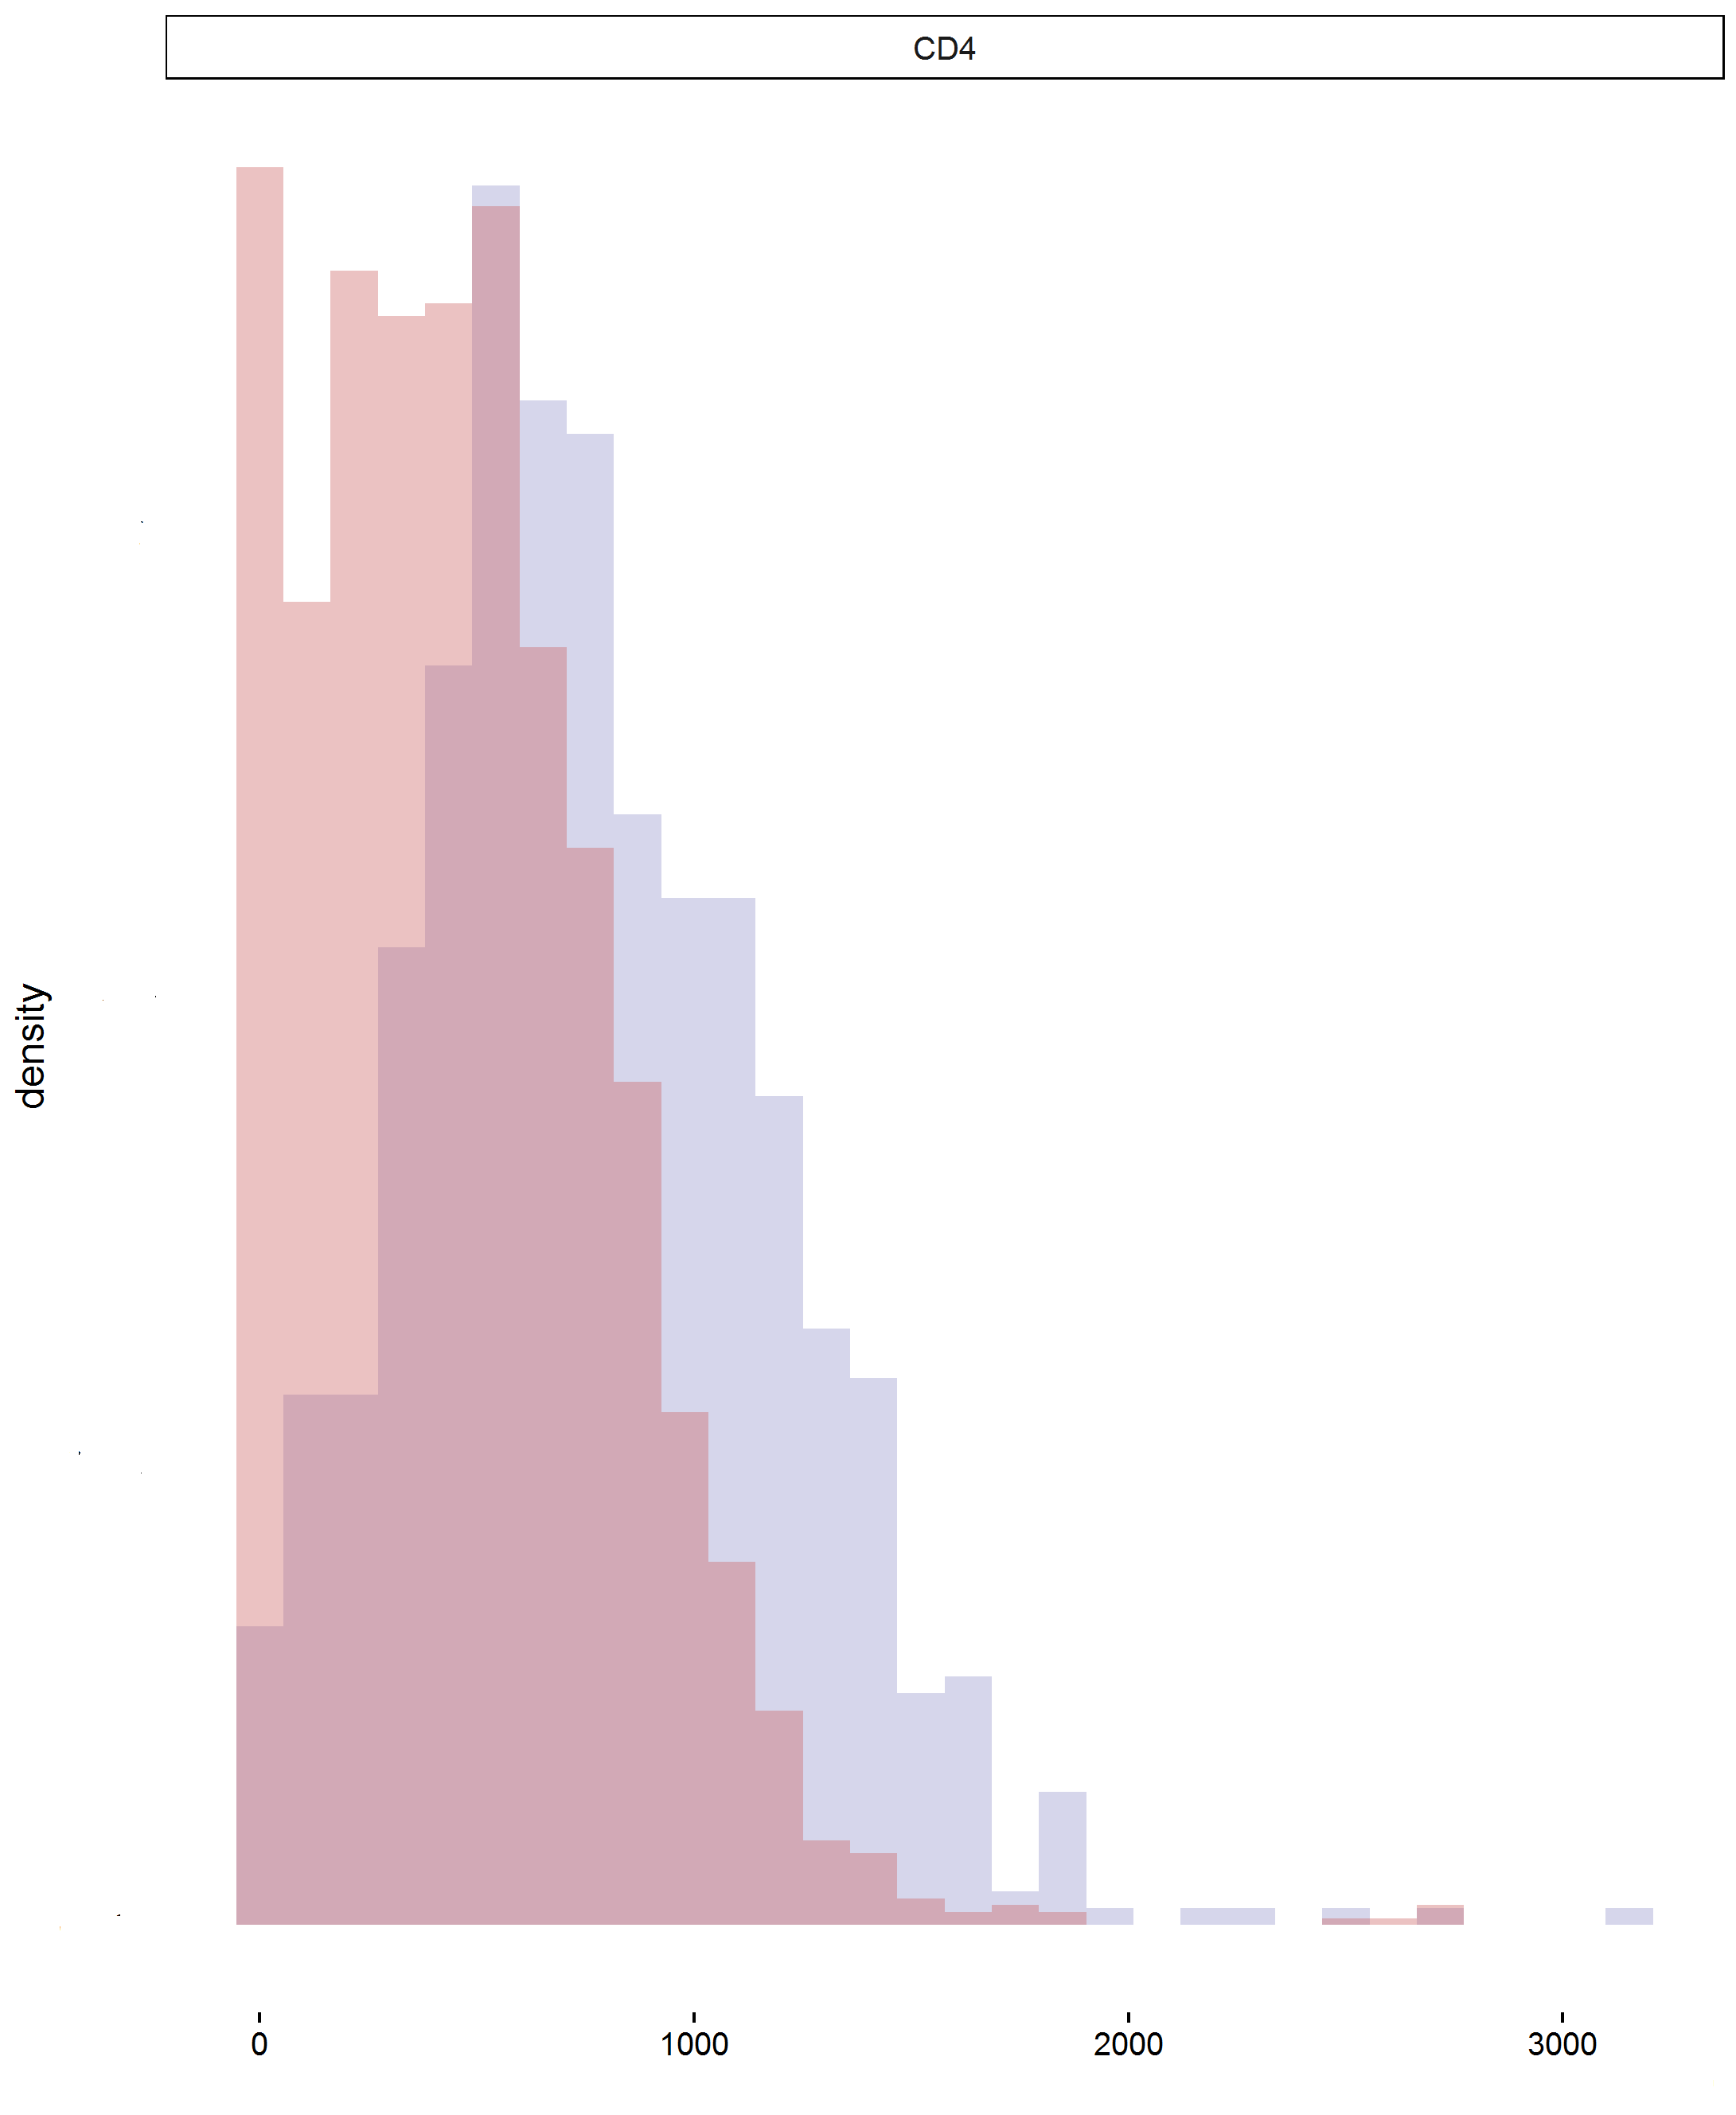
\includegraphics[scale=.25]{fig4.png}
\end{frame}
\begin{frame}
  \begin{columns}
    \begin{column}{.5\textwidth}
  \begin{tabular}{c | c | c}
    & control & case\\
    \hline&&\\
    obs. \# 1 & $X_1$ & \\
    \vdots & \vdots & \\
    obs. \# k & $X_{k}$ &\\
      obs. \# k+1 &  & $Y_{k+1}$\\
     \vdots & & \vdots\\
    obs. \# \I &  & $Y_{\I}$\\
  \end{tabular}
\end{column}
\begin{column}{.5\textwidth}
  The AUC is the probability that an observation drawn from a
  negative/control/non-diseased subject is less than an independent
  observation from a positive/case/diseased subject.
  $$\text{AUC}=\P(X < Y)=\E(F_X(Y))$$
  $$\widehat{\text{AUC}}=\frac{1}{k(\I-k)}\sum_{i,j}\{X_i<Y_j\}$$
\end{column}
\end{columns}
\end{frame}

\begin{frame}
  % \begin{columns}
  %   \begin{column}{.5\textwidth}
  \centering
  \begin{tabular}{c | c | c}
    & control & case\\
    \hline&&\\
    obs. \# 1 & $(X_{11},\ldots,X_{1m_1})$ & $(Y_{11},\ldots,Y_{1n_1})$\\
    \vdots & \vdots & \vdots\\
    obs. \# \I & $(X_{\I1},\ldots,X_{\I m_{\I}})$ & $(Y_{\I1},\ldots,Y_{\I n_{\I}})$\\
  \end{tabular}
% \end{column}
% \begin{column}{.5\textwidth}
%   picture of our data. add clusters+correlations. clustered version/ population auc. phi notation. give statitsic. O(1/I) bias.
  \begin{itemize}    
  \item Assume iid observations. Denote AUC between cluster $i$ controls and cluster $j$ cases as
    \begin{columns}
      \begin{column}{.5\textwidth}
        $$ \phi_{ij}=\frac{1}{m_in_k}\sum_{j=1}^{m_i}\sum_{l=1}^{n_k}\{X_{ij}<Y_{kl}\}$$
      \end{column}
      \begin{column}{.3\textwidth}
        $$\phi=
        \begin{pmatrix}
          \phi_{11} & \ldots &  \phi_{1\I}\\
          \vdots & \vdots & \vdots\\
          \phi_{\I1} & \ldots &  \phi_{\I\I}
        \end{pmatrix}$$
      \end{column}
    \end{columns}
  \item Generalize AUC to clustered data as
  $$\theta=\text{AUC}=\E(\phi_{ij}), i\neq j$$
  $$\hat\theta=\widehat{\text{AUC}}=\auchat=\frac{1}{\I^2}\sum_{i,j}\phi_{ij}$$
\end{itemize}
% \end{column}
% \end{columns}
\end{frame}
\begin{frame}
  % repeat fig of data
  \begin{itemize}
  \item markers: longitudinal measurements of tumour antigens (CEA,
    CA15-3, TPS) as markers, response: progression/non-progression of breast
    cancer (Emir 2000)

  \item markers: two measurements of the distortion product otoacoustic
    emissions taken from the left and right eyes ((think this should
    be ears)) of each patient, response: neonatal hearing impairment
    (Wu 2019)

  \item markers: longitudinal measurements of levels of vascular
    enothelial growth factor and a soluble fragment of Cytokeratin 19,
    response: progression/non-progression of non-small cell lung
    cancer (Wu, Wang 2011)
   \end{itemize}
 \end{frame}
 
 \begin{frame}
   \begin{itemize}
 \item Fix cluster sizes $m_i=m,n_j=n,1\le i,j \le \I$
   
 \item   Obuchowski '97 estimates the variance of $\auchat=\widehat{\text{AUC}}$ as
  \begin{align}
   \hat\sigma^2_{obu}&=\frac{1}{\I(\I-1)}\sum_i(\rowmean{i}+\colmean{i}-2\auchat)^2\\
                     &=\frac{1}{\I}\widehat{var}(\rowmean{i}+\colmean{i})\\
  (\auchat-\E(\auchat))/\hat\sigma_{obu} &\leadsto N(0,1)
  \end{align}
   \item Alternatively: Use the bootstrap. Sample the iid
   clusters without replacement, compute $\auchat$ on the sample,
   repeat. Take the sample variance of the resulting $\auchat$'s.
 \end{itemize}
\end{frame}
\begin{frame}
  \centering
  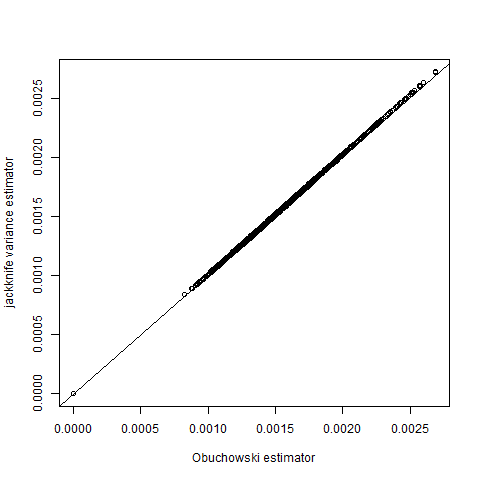
\includegraphics[scale=.5]{fig9.png}
\end{frame}
\begin{frame}
  \centering
  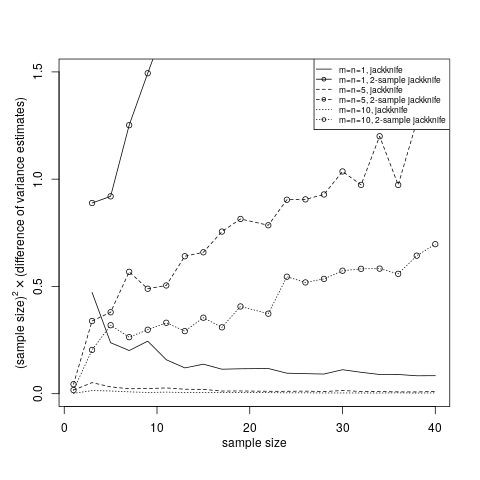
\includegraphics[scale=.5]{fig1.png}
\end{frame}
% \begin{frame}
% asymptotic result
% \end{frame}

% \section{Main}

\begin{frame}
  Objective is 
  \begin{align}
    \speak{!!!((I-1)) in denominator}
    &\propto \frac{2\I-1}{\I^2}\sum_j(\rowmean{j} + \colmean{j} - 2\hat{\theta})^2 \\
    &- \frac{2}{\I}\sum_j\left(\rowmean{j} + \colmean{j} - 2\hat{\theta}\right)\left(\phi_{jj}-\frac{\tr(\phi)}{\I}\right) \\
      &+\text{lower order terms}
  \end{align}
\end{frame}
\begin{frame}
  \begin{itemize}
    \item When $m=n=1$, clusters can be ordered by $y_i$ (``case'') observations
    \item $\phi_{ij}=\{x_i<y_j\}$, e.g., $\phi=
      \begin{pmatrix}
        0 & 1 & 1\\
        0 & 0 & 1\\
        1 & 1 & 1
      \end{pmatrix}$
      
    \item $a_i:=\phi_{i\cdot}$ the row sums, $0\le a_i\le \I$
      $F_a(x)=\sum_{i=1}^{\I}\{a_i\le x\}$ the observed CDF of the $a_i$
      objective is
      \begin{align}
        &\propto \frac{1}{\I^2}\sum_ia_i^2 +\frac{2}{\I}a_i(1-F_a(\I-i))\\
        &+\sum_i(1-F_a(\I-i))^2+\frac{2}{\I^2}(\sum_ia_i)(\sum_i(1-F_a(\I-k)))\\
        &-\sum_i(1-F_a(\I-k))\{a_i>\I-i\}-\frac{4}{\I^3}(\sum_ia_i)^2\\
        &-\frac{1}{\I}\sum_ia_i\{a_i>\I-i\}
      \end{align}
      % \speak{would like to reduce to m=n=1 case, but not convex}
  \end{itemize}
\end{frame}
\begin{frame}
  View the objective as a quadratic form $\Q$ in the $\I^2$ entries of $\phi$
    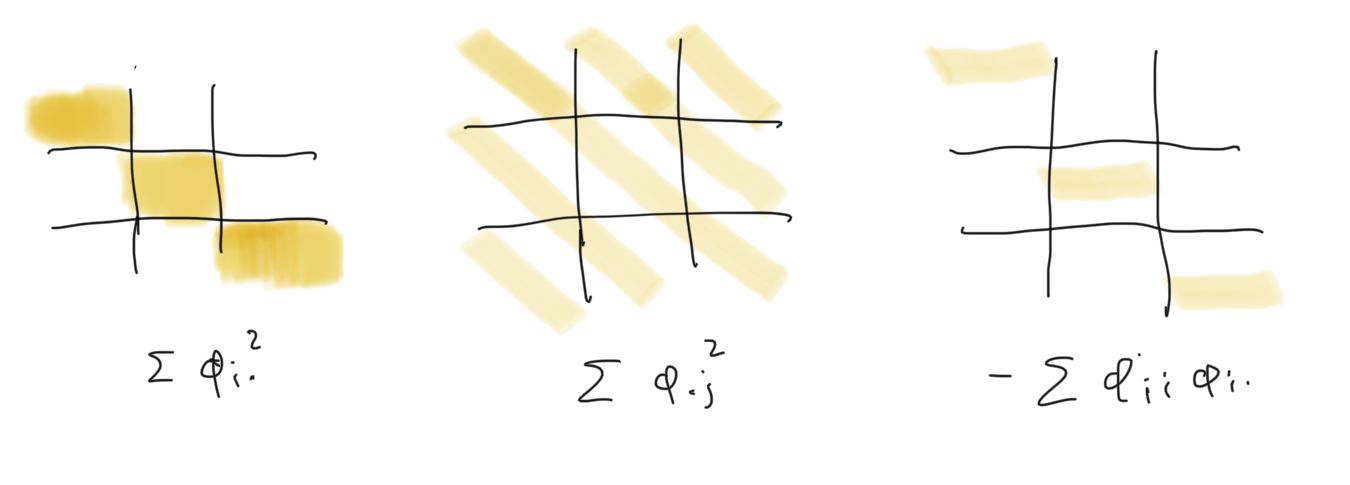
\includegraphics[width=\textwidth]{fig10.png}
\end{frame}
\begin{frame}
  \begin{columns}
    \begin{column}{.5\textwidth}
      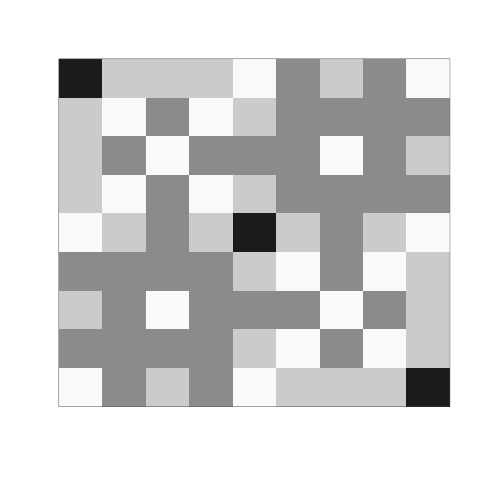
\includegraphics[width=\textwidth]{fig6.png}
    \end{column}
    \begin{column}{.5\textwidth}
      \begin{itemize}
      \item $\I^2$ $\I\times\I$ blocks
      \item $Q_{pqrs}=\frac{1}{\I^2}(\{p=q\}+\{r=s\}+\{q=r\}+\{p=s\}+\{s=q\}+\{p=r\})-\frac{1}{2\I}(\{p=q=r\}+\{p=q=s\}+\{p=r=s\}+\{q=r=s\})-\frac{4}{\I^3}$ is symmetric in $p,q,r,s$
      \item $\Q$ is symmetric about the diagonal, anti-diagonal, and
        $180^\circ$ rotations
      \end{itemize}
    \end{column}
  \end{columns}
\end{frame}
\begin{frame}
  \begin{columns}
    \begin{column}{.5\textwidth}
      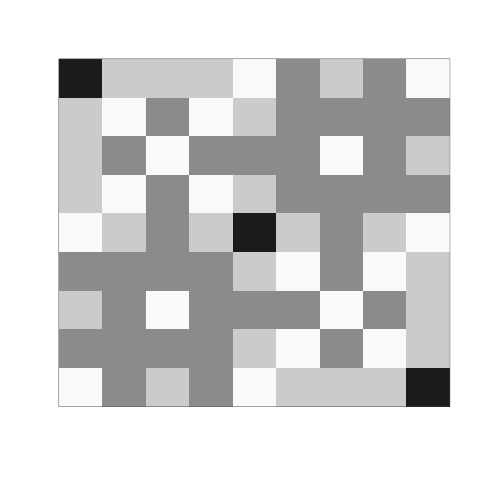
\includegraphics[width=\textwidth]{fig6.png}
    \end{column}
    \begin{column}{.5\textwidth}
      \begin{itemize}
      \item $\Q=(P\otimes P)^t\Q(P\otimes P)$ for a permutation matrix
        $P$ (shuffling iid clusters)
      \end{itemize}
    \end{column}
  \end{columns}
  \speak{some consequences of symmetry. decision to use quad form--obscures symmetries in the problem.shows up in nullspace.}    
\end{frame}
% \begin{frame}
%   \begin{itemize}
%   \item blocks and $\Q$ itself are symmetric about the diagonal, anti-diagonal, and $180\deg$ rotations ((another picture of quad form here?))
%   \item $\Q=(P\otimes P)^t\Q(P\otimes P)$ (shuffling iid clusters)
%   \end{itemize}
%   \speak{some consequences of symmetry. decision to use quad form--obscures symmetries in the problem.shows up in nullspace.}    
% \end{frame}
\begin{frame}
  % operator theorem incl characteristic eqn. scaled difference of two projection matrices onto $\I-1$ dimensional subspaces.
  \begin{itemize}
  \item characteristic polynomial  $x^{\I^2-2(\I-1)}(2x^2-\frac{\I-2}{\I^2})^{\I-1}$
  \item $\Q^{2k+1}=\eigval^{2k}\Q$ and $\Q^{2k}=\eigval^{2(k-1)}\Q^2$
  \item $\Q$ is the scaled difference of two orthogonal  projection matrices onto two $\I-1$ dimensional subspaces $$\Q = \lambda(\Q_1-\Q_2)$$
  \end{itemize}
\end{frame}
\begin{frame}
  (aside) Relate the traces of powers $t_j=\tr(\Q^j)$ to the coefficients $c_j$ of the characteristic polynomial
  \begin{align}
    c_1&=t_1\\
    c_2&=\frac{1}{2}(t_1^2-t_2)\\
    c_3&=-\frac{1}{6}t_1^3+\frac{1}{2}t_1t_2-\frac{1}{3}t_3\\
    &\vdots
  \end{align}
  With our traces and coefficients,
  \begin{align}
    &-\frac{\I-1}{k}+\frac{(\I-1)^2}{2!}\sum_{i_1+i_2=k}\frac{1}{i_1i_2} - \frac{(\I-1)^3}{3!}\sum_{i_1+i_2+i+3=k}\frac{1}{i_1i_2i_3}+\ldots\\
    &+(-1)^{k-1}\frac{(\I-1)^{k-1}}{(k-1)!} = (-1)^{\I+k}{\I-1\choose k}
  \end{align}
\end{frame}
\begin{frame}
  (aside)
i.e. $(-1)^k{\I-1\choose k}$ is the coefficient of $x^k$ in $$\sum_{m=1}^{\I-1}(-1)^m\frac{(\I-1)^m}{m!}(x+x^2/2+x^3/3+\ldots+\frac{x^{\I-1}}{\I-1})^m.$$ 
  \begin{align}
    \sum_{i_1+\ldots+i_m}\frac{1}{i_1\cdot\ldots\cdot i_m}=\frac{|s^k_m|}{k!}\\
  \end{align}
  with $|s^k_m|$ the Stirling number of the first kind
  \begin{align}
    x^{\underline{k}}=\frac{x!}{(x-k)!}=\sum_{m=1}^k s^k_m x^m
  \end{align}
  e.g.
  \begin{align}
    x^{\underline{4}}=x(x-1)(x-2)(x-3)=x^4-6x^3+11x^2-6x
  \end{align}
\end{frame}
\begin{frame}
  \begin{columns}
    \begin{column}{.5\textwidth}
      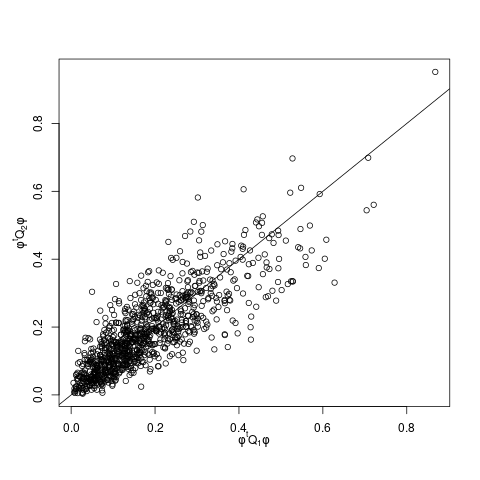
\includegraphics[width=\textwidth]{fig7.png}
      \speak{haven't moved very far away from the original problem. started with a difference of psd operators. OTOH we have found a common scale factor, and these are very simple psd operators (projections).}
    \end{column}
    \begin{column}{.5\textwidth}
      \begin{itemize}
      \item nullspace has dimension $\I^2-2(\I-1)$
      \item need $\Q$-null vectors $v$, $(v,\Q v)=0$, and relate these to the structure of $\phi$
      \end{itemize}
    \end{column}
  \end{columns}
\end{frame}

\begin{frame}
  (Aside)
  \begin{columns}
    \begin{column}{.5\textwidth}
      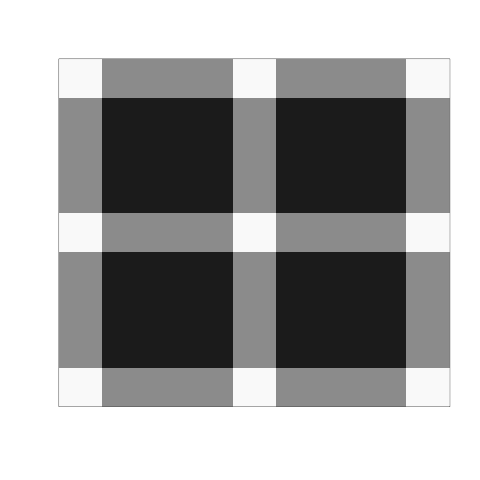
\includegraphics[width=\textwidth]{fig8.png}
    \end{column}
    \begin{column}{.5\textwidth}
      \begin{itemize}
      \item Element-wise ratio $\Q_2/\Q_1$ only takes 3 values: $-1,r_{\I},1/r_{\I}$\\
        % \hspace{.1in}
        \begin{tabular}{c | c}
          $\I$ & $r_{\I}$\\
          \hline
          3 &  $17+12\sqrt{2} = \epsilon_0(2)^4$\\
          4 &  $Inf$\\
          5 &  $49+20\sqrt{6} = \epsilon_0(6)^2$\\
          6 &  $17+12\sqrt{2} = \epsilon_0(2)^4$\\% (= case 3)\\
          7 & $19.7270...$\\
          8 &  $7+4\sqrt{3} = \epsilon_0(3)^2$\\
          9 & $10.8679...$\\
          10 & $ 9$\\
          12 &  $7/2+3/2\sqrt{5} = \epsilon_0(5)^4$\\
          20 &  $4$\\
        \end{tabular}
      \end{itemize}
    \end{column}
  \end{columns}
\end{frame}


% \begin{frame}
% aside:  
% \end{frame}
\begin{frame}
  Mutually $\Q$-orthogonal vectors include (vectorizations of)
  \begin{itemize}
  \item constant row/column $\phi$ e.g.
    $\begin{pmatrix}
      1 & 0 & 0\\
      1 & 0 & 0\\
      1 & 0 & 0
    \end{pmatrix}$,
    $\begin{pmatrix}
      0 & 0 & 0\\
      1 & 1 & 1\\
      0 & 0 & 0
    \end{pmatrix}$
  \item constant diagonal $\phi$ e.g.
        $\begin{pmatrix}
      1 & 0 & 0\\
      0 & 1 & 0\\
      0 & 0 & 1
    \end{pmatrix}$
  \item upper triangular $\phi$ in $N(\Q)$
    $\begin{pmatrix}
      1 & 1 & 1\\
      0 & 1 & 1\\
      0 & 0 & 1
    \end{pmatrix}$
  \end{itemize}
  i.e., stack bases for the above to form a matrix $B$, then $B^tQB=0$
\end{frame}
\begin{frame}
  \begin{itemize}
  \item  structure of matrix given by $\phi_{ij}=\mathbbm{E}_{}F_{X_j}(Y_j)$
  
  \item  can't order $y$ (case) clusters when $n>1$
  
  \item  but $\phi$ is a mixture of totally ordered vectors $0\le v_1\le v_2\le\ldots\le v_n\le m$
  \begin{align}
    \phi=\frac{1}{mn}    \begin{pmatrix}
      \vdots & \vdots & & \vdots \\
      v_1 & v_2 & \cdots & v_{\I n}\\
      \vdots & \vdots & & \vdots
    \end{pmatrix}
                          \underset{\textstyle \text{col sums}=n}{
                          \begin{pmatrix}                            
                            1 & 0 &  & 0\\
                            0 & 1 &  & 1\\
                            \vdots&\vdots & \cdots &\vdots \\
                            1 & 0 &  & 1\\
                          \end{pmatrix}}
     \text{row sums}=1\\
  \end{align}
\end{itemize}
\end{frame}
\begin{frame}
  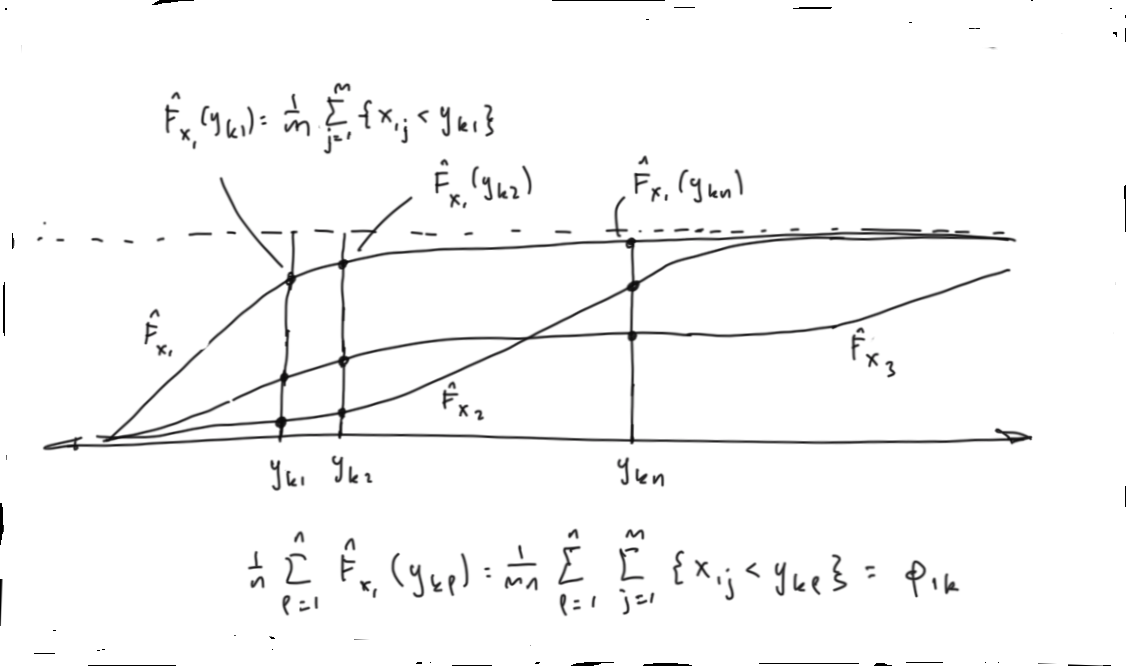
\includegraphics[width=\textwidth]{fig13.png}
\end{frame}
\begin{frame}
  \begin{align}    
    &mn\phi=\\
    &\scriptstyle{\text{row sums}=m}
  \underset{\text{col sums} = 1}{  \begin{pmatrix}
      0 & 1 &\cdots & 1 \\
      1 & 0 &\cdots & 0\\
       &  & \vdots & \\
       0 & 0 &\cdots & 0
    \end{pmatrix}}
                      \begin{pmatrix}
                        1 & 1 & \cdots & 1\\
                        0 & 1 & \cdots & 1\\
                        & & \ddots & \\
                        0 & 0 & \cdots & 1
                      \end{pmatrix}
    \underset{\text{col sums}=n}{
                          \begin{pmatrix}                            
                            1 & 0 &  & 0\\
                            0 & 1 &  & 1\\
                            \vdots&\vdots & \ldots &\vdots \\
                            1 & 0 &  & 1\\
                          \end{pmatrix}}
    \scriptstyle{\text{row sums}=1}\\
    % &vec(\phi)=\underset{\substack{\I\times\I(m+n)}}{\tilde{P_1}}\otimes\underset{\I\times\I(m+n)}{\tilde{P_2}}\underset{\substack{\I(m+n)\times\\\I(m+n)}}{T}
  \end{align}
  If the 1st and 3rd matrices are permutation matrices, $\phi$ is in the nullspace of $\Q$
\end{frame}
\begin{frame}
  \begin{itemize}
    \item Project $\phi$ onto a subset of the $\Q$-null vectors and examine
      residual
      \item Let $P=(1,\ldots,\I)$ and $\colmean{p}=(\colmean{1},\ldots,\colmean{\I})$
  \begin{align}
    \V(\colmean{p})-\cov^2(\colmean{p},\frac{P}{sd(P)})
  \end{align}
\item $D(x)=|\cov((x_{(1)},\ldots,x_{(\I)}),\frac{P}{sd(P)})|$ can be viewed as a measure of statistical dispersion of $(x_1,\ldots,x_{\I})$
  \begin{align}
    D(ax+b)=|a|D(x)+b
  \end{align}
\end{itemize}
\end{frame}
\begin{frame}
  \begin{itemize}
  \item $\V(x)-D^2(x)\ge 0$, equals $0$ when $x\propto (1,\ldots,\I)$ i.e., $(x_{1},\ldots,x_{\I})$ are evenly spaced
  \item conjecture it is maximized for $0\le x\le 1$ when $x=(0,0,\ldots,0,1)$, where the value is $O(1/\I)$
  \item \begin{itemize}
      \item Maximizing a postive semi-definite function over a
        polytope $0\le x_1\le\ldots\le x_{\I}\le 1$
      \item Maximum occurs at a
        corner point given by the intrsection of $\I$ hyperplanes
        \item $\I$ of the $\I+1$ restrictions
    $0\le x_1, x_1\le x_2,\ldots,x_{\I-1}\le x_{\I}, x_{\I}\le 1$ are
    active
  \item Only need to check $x$ of the form  $(0,\ldots,0,1,\ldots,1)$.
  \end{itemize}
\end{itemize}
\end{frame}
\begin{frame}
  The difference between the jackknife and Obuchowski variance estimates is $O(1/\I^2)$ when $\phi$ is lower right triangular
\end{frame}


\begin{frame}
  Future work
  \begin{itemize}
  \item stochastic result needed or sharpen constants
  \item   varying cluster sizes
  \end{itemize}
\end{frame}
% \begin{frame}

%   \textbf{Causal framework:} There are no unmeasured confounders; we can obtain
%   the causal effect by controlling for the known confounder.

% \end{frame}

\end{document}
